\documentclass[11pt]{amsart}

\textwidth 6.3in

\evensidemargin=-0.1cm \oddsidemargin=-0.1cm

\textheight 8.1in

\usepackage{comment}
\usepackage{listings}
\usepackage{xcolor}
\usepackage{enumitem}
\usepackage{url}
\usepackage{graphicx}
\usepackage{amsmath}

% Configure code listings
\lstset{
    basicstyle=\ttfamily\small,
    breaklines=true,
    frame=single,
    backgroundcolor=\color{gray!10},
    keywordstyle=\color{blue}\bfseries,
    commentstyle=\color{green!60!black},
    stringstyle=\color{red},
    showstringspaces=false,
    tabsize=4
}


\begin{document}

\begin{center}
\huge HW3 \\
50pts \\

\Large Posted Friday, October 3

\Large Due Thursday, October 16

\normalsize
\end{center}

Submit written part in \texttt{HW3Solutions.pdf} and code in \texttt{predictive\_rec\_descent.py} and \texttt{predictive\_rec\_descent.pl}. Submission size limit is 2.5MB. 

\vspace{0.2in}

\noindent{\bf Problem 1} (20pts). Consider the pseudocode with nested subroutines:


\begin{verbatim}
procedure main
     g : integer
       
     procedure B(a : integer) 
          x : integer

          procedure A(x : integer)
               g := x
                  
          procedure R(m : integer)
               write_integer(x)
               x /:= 2 -- integer division 
               if x > 1
                   R(m + 2)
               else
                   A(m + 1)
              
          -- body of B
          x := a * a
          R(1)
          
     -- body of main
     B(3)
     write_integer(g)   
                      
\end{verbatim}

\begin{itemize}

\item[a)] (5pts) What does the program print under static scoping? 

\begin{verbatim}
 Output:  9
          4
          2
          6
\end{verbatim}

\newpage

\item[b)] (5pts) Show the frames on the stack when A has just been called assuming static scoping rules. Show the static and dynamic links of each frame, as well as the local variables and their values right after the assignment \texttt{g := x}. Explain how \texttt{A} finds \texttt{g}.

\vspace{0.2in}

\begin{center}
     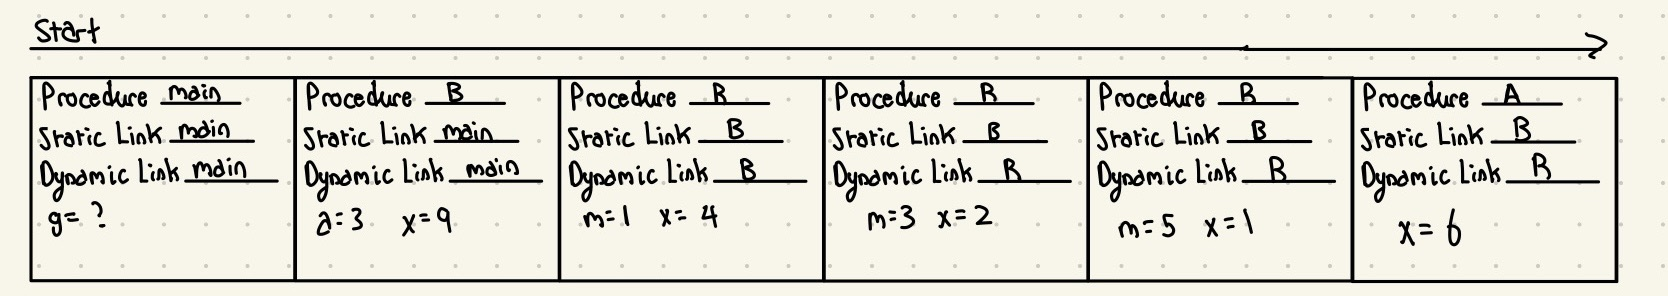
\includegraphics[width=0.9\textwidth]{IMG_0084.jpg}
\end{center}

\vspace{0.2in}


\item[c)] (5pts) Now, what does this program print under dynamic scoping?

\begin{verbatim}
 Output:  9
          4
          2
          1
\end{verbatim}

\item[d)] (5pts) Explain how \texttt{R} finds \texttt{x} under dynamic scoping rules.

\vspace{0.1in}

Under dynamic scoping, when \texttt{R} executes write\_integer(\texttt{x}), it looks for \texttt{x} in this order up the call chain:

\vspace{0.1in}

1. It's own frame - \texttt{R}'s local vars - if not found, then move onto

2. The caller's frame - \texttt{B}'s local vars - if not found, then onto

3. The caller's caller's frame - \texttt{main}'s local vars, and so on

\vspace{0.1in}

Here, R does not have its own x.
So it searches up the call chain and finds x in the B frame,
which it then uses continuously to reference, modify, and print out.

\end{itemize}


\vspace{1in}

\newpage

\noindent{\bf Problem 2} (30pts). The grammar below
generates boolean expressions in prefix form:

\[\begin{array}{lll}
\mathit{start} & \rightarrow & \mathit{expr} \ \texttt{\$\$} \\
\mathit{expr} & \rightarrow & \texttt{or}\ \mathit{expr} \ \mathit{expr} \ | \ \texttt{and} \ \mathit{expr} \ \mathit{expr} \ | \ \texttt{not}\ \mathit{expr} \ | \ {\texttt {id}} \\
\end{array}\]

\begin{itemize}

\item[a)] (5pts) Write an attribute grammar (in pseudocode) to translate expressions into fully parenthesized infix form. For example, 
expression \texttt{and and a or b c d} turns into the following fully parenthesized expression \texttt{((a and (b or c)) and d)}. 
\vspace{0.2in}

{\small
\hspace*{-.5cm}
\begin{tabular}{r@{\hspace{1em}}c@{\hspace{2em}}l}
1. & $\text{expr} \to \text{or expr}_1 \text{ expr}_2$ 
   & $\text{expr.val} := "(" + \text{expr}_1.\text{val} + " \text{ or } " + \text{expr}_2.\text{val} + ")"$ \\[6pt]
2. & $\text{expr} \to \text{and expr}_1 \text{ expr}_2$ 
   & $\text{expr.val} := "(" + \text{expr}_1.\text{val} + " \text{ and } " + \text{expr}_2.\text{val} + ")"$ \\[6pt]
3. & $\text{expr} \to \text{not expr}_1$ 
   & $\text{expr.val} := "( \text{not } " + \text{expr}_1.\text{val} + ")"$ \\[6pt]
4. & $\text{expr} \to \text{id}$ 
   & $\text{expr.val} := \text{id.s}$ \\
\end{tabular}
}
\vspace{0.2in}


\item[b)] (5pts) Now write an attribute grammar (in pseudocode again) to translate the expressions into \emph{parenthesized} 
expressions in infix form \emph{without redundant parentheses} assuming the standard convention: unary \texttt{not} has highest precedence, 
followed by \texttt{and}, followed by \texttt{or}, and \texttt{and} and \texttt{or} are left-associative. For example, the above expression 
turns into \texttt{a and (b or c) and d}. \emph{Hint:} Assign a precedence attribute $\mathit{prec}$ to operators and expressions. 
In part c) and part d) you will code your solution respectively in Python and in Prolog. 

\vspace{0.1in}

First, let's assign two synthesized attributes to the expressions/terminals:

\vspace{0.1in}

\begin{itemize}
     \item[1.] \texttt{val} - the resulting infix string
     \item[2.] \texttt{prec} - it's precendence (higher number means higher precedence)
\end{itemize}

\vspace{0.1in}

Then, synthesize precedences to the operators/terminals(\small{prec(operator)})(Higher number means higher precedence):

\vspace{-.09in}

\[
\begin{array}{cccc}
\text{prec(id)} = 4 & \text{prec(not)} = 3 & \text{prec(and)} = 2 & \text{prec(or)} = 1
\end{array}
\]

\vspace{0.1in}

Now, let's write the attribute grammar with helper functions $\text{paren}_L$(E, p), $\text{paren}_R$(E, p), and $\text{paren}_{un}$(E, p) that adds parentheses to the left, right, or unary expression E if its precedence is lower than p.:

\vspace{0.1in}

Helper functions:

\[
\operatorname{paren}_L(E,p)=
\begin{cases}
( E.\mathrm{val} ) & \text{if } E.\mathrm{prec} < p, \\
E.\mathrm{val}    & \text{otherwise.}
\end{cases}
\]
\[
\operatorname{paren}_R(E,p)=
\begin{cases}
( E.\mathrm{val} ) & \text{if } E.\mathrm{prec} \le p, \\
E.\mathrm{val}     & \text{otherwise.}
\end{cases}
\]

\[
\operatorname{paren}_{\mathrm{un}}(E,p)=
\begin{cases}
( E.\mathrm{val} ) & \text{if } E.\mathrm{prec} < p, \\
E.\mathrm{val}     & \text{otherwise.}
\end{cases}
\]
CONTINUED ON NEXT PAGE

\newpage

Attribute Grammer:

\vspace{0.2in}

{\small
\hspace*{-.5cm}
\begin{tabular}{r@{\hspace{1em}}c@{\hspace{2em}}l}
1. & $\text{expr} \to \text{or expr}_1 \text{ expr}_2$ 
   & $\text{expr.prec} := 1$ \\
   & & $\text{expr}.\text{val} := \text{paren}_L(\text{expr}_1, 1) \text{ } + \text{ " or " } + \text{ paren}_R(\text{expr}_2, 1)  $\\[6pt]
2. & $\text{expr} \to \text{and expr}_1 \text{ expr}_2$ 
   & $\text{expr.prec} := 2$ \\
   & & $\text{expr}.\text{val} := \text{paren}_L(\text{expr}_1, 2) \text{ } + \text{ " and " } + \text{ paren}_R(\text{expr}_2, 2)  $\\[6pt]
3. & $\text{expr} \to \text{not expr}_1$ 
   & $\text{expr.prec} := 3$ \\
   & & $\text{expr}.\text{val} := \text{"not "}  + \text{ paren}_{un}(\text{expr}_1, 3)$\\[6pt]
4. & $\text{expr} \to \text{id}$ 
   & $\text{expr.prec} := 4$ \\
   & & $\text{expr}.\text{val} := \text{id.s}$ \\[6pt]
\end{tabular}
}



\end{itemize}

\end{document}
